\documentclass{sig-alternate}

\usepackage{graphicx,amsmath,amssymb,epsfig}
%\usepackage{algorithm,algorithmic}
\usepackage{url}
\newcommand{\CodeIn}[1]{{\small\texttt{#1}}}
\usepackage{subfigure}

\begin{document}
%
% --- Author Metadata here ---
\conferenceinfo{ICSE}{'10, May 2-8, 2010, CAPE TOWN, SOUTH AFRICA}
%\CopyrightYear{2007} % Allows default copyright year (200X) to be over-ridden - IF NEED BE.
%\crdata{0-12345-67-8/90/01}  % Allows default copyright data (0-89791-88-6/97/05) to be over-ridden - IF NEED BE.
% --- End of Author Metadata ---

\title{ Test Selection via Mining Common Operational Models }

\numberofauthors{3}
\author{
% 1st. author
\alignauthor
Wujie Zheng\\
       \affaddr{Department of Computer Science \& Engineering}\\
       \affaddr{The Chinese University of Hong Kong}\\
       \email{wjzheng@cse.cuhk.edu.hk}
% 2nd. author
\alignauthor Michael R. Lyu\\
       \affaddr{Department of Computer Science \& Engineering}\\
       \affaddr{The Chinese University of Hong Kong}\\
       \email{lyu@cse.cuhk.edu.hk}
% 3rd. author
\alignauthor Tao Xie\\
       \affaddr{Department of Computer Science}\\
       \affaddr{North Carolina State University}\\
       \email{xie@csc.ncsu.edu}
}
\maketitle

\begin{abstract}
In automated testing, especially test generation in the absence of
specifications, a large amount of manual effort is spent on
test-result inspection. Test selection helps to reduce this effort
by selecting a small subset of tests that are likely to reveal
faults. A promising test-selection approach is to dynamically mine
operational models as potential test oracles and then select tests
that violate them. Existing work adopting this approach mines
operational models based on dynamic invariant detection. In this
paper, we propose to mine common operational models, which are often
but not always true in all observed traces, from a (potentially
large) set of unverified tests. Specifically, our approach collects
branch coverage and data value bounds at runtime and then mines
implication relationships between branches and constraints of data
values as potential operational models after running all the tests.
Our approach then selects tests that violate the mined common
operational models for result inspection. We have evaluated our
approach on a set of programs, compared with previous
code-coverage-based, clustering-based, dynamic-invariant-based, and
random selection approaches. The experimental results show that our
approach can effectively reduce the number of tests for result
inspection while revealing most of the faults.
%The experimental results
%show that our approach is effective for test selection.


\end{abstract}

%% A category with the (minimum) three required fields
%\category{D.2.5}{Software Engineering}{Testing and Debugging}
%%\category{D.2.8}{Software Engineering}{Metrics}[complexity measures,
%%performance measures]
%
%\terms{Reliability, Experimentation}
%
%\keywords{Software testing, Test selection}

\section{Introduction} \label{sec:intro}

% the problem description
It is labor-intensive to manually generate a large set of test
inputs and verify their outputs. Recently, there have been various
practical approaches on automatic test-input
generation~\cite{Pacheco07, Sen05, Visser04}. However, test-result
inspection still remains a largely manual task. Given \emph{a
priori} specification, developers can reduce this manual effort by
selecting test inputs (in short as \emph{tests}) using specification
coverage criteria~\cite{Chang99}. But it is uncommon to have \emph{a
priori} specification in practice. Sometimes developers may use
general test oracles based on memory monitoring tools such as
Valgrind ~\cite{Nethercote07}. But these oracles are limited in
checking specific kinds of faults. It is highly demanded to develop
practical test-selection techniques, which can select a small subset
of tests that are likely to reveal faults.


A promising test-selection approach is to dynamically mine
operational models as potential test oracles and then select tests
that violate them. Existing approaches such as Jov~\cite{Xie03} and
Eclat~\cite{Pacheco05} mine dynamic invariants using
Daikon~\cite{Ernst01} from a set of manually written passing unit
tests whose results are verified with manually written assertions.
Due to nontrivial effort for writing the assertions, the number of
these existing passing unit tests is often limited. Therefore, the
mined dynamic invariants could be noisy and thus many model
violations could be false positives. The operational difference
approach~\cite{Harder03} starts with an empty test suite and
repeatedly adds new tests if they violate the invariants mined from
the previously selected tests. As the number of previously selected
tests is also limited, this approach faces the same problem of
producing many false positives. DIDUCE~\cite{Hangal02} mines
operational models from normal execution of long-running
applications and relaxes the models gradually. At the beginning of a
program run, many presumed operational models may be violated and a
violation that reveals a fault can be overwhelmed by the
false-positive noise.

In this paper, we propose to mine common operational models, which
are often but not always true in all observed traces, from a
(potentially large) set of unverified tests. A program that is not
of poor quality should pass most of the tests. So the common
operational models mined from a large set of unverified tests may be
similar to the true operational models and their violations are
likely to reveal faults. By using the information of all the
unverified tests at hand, our approach can avoid the noise caused by
a small number of data samples, without requiring a large set of
verified tests. As a common operational model is not always true
over the whole set of tests, the type of Daikon inference techniques
does not work anymore. Alternatively, we may generate and collect
all the potential models at runtime (instead of immediately
discarding any violated potential models) and evaluate them after
running all the tests. However, such an approach can incur high
runtime overhead if Daikon-like operational models, which are in a
large number, are used.






To mine common operational models efficiently, we propose an
approach based on mining control rules and data rules. A control
rule is an implication relationship between branches, and a data
rule is an implicit constraint of the variable values. Specifically,
our approach collects branch coverage and data value bounds at
runtime using the Cooperative Bug Isolation (CBI)
tools~\cite{Liblit04}. Our approach then mines control rules and
data rules as potential operational models after running all the
tests. The likelihood of a common operational model to be a true
oracle is evaluated using the concept of confidence, i.e., the ratio
of the number of tests that satisfy the model over the number of
tests that satisfy or violate the model. When a model's confidence
is not equal to 1, the higher the model's confidence is, the more
suspicious its violations are in revealing a fault. Finally, our
approach selects a small subset of tests that violate the mined
common operational models for result inspection.


To illustrate what a common operational model may look like and how
its violation is useful for indicating faults, we present an example
in Figure~\ref{fig:example1}. The example is a faulty version of
grep 2.3, which is downloaded from the Software Infrastructure
Repository (SIR)~\cite{SIR}. grep is a GNU utility that searches the
input files for lines containing a match to a given pattern list.
When grep finds a match in a line of a text file, it copies the line
to the standard output. But if the input file is a binary file, it
normally\footnote{By default, binary files are not treated as text
files} outputs either a one-line message saying that a binary file
matches, or no message if there is no match. Furthermore, given the
option ``--quiet'', grep should not write anything to the standard
output.

\begin{figure}[t]
\begin{center}
  \includegraphics[angle=0,width=0.4\textwidth]{figs/example11.eps}
  \centering
  \caption{Faulty code of the grep program}
  \label{fig:example1}
\end{center} \vspace{-0.2in}
\end{figure}



In Line 1, $\CodeIn{always\_text}$ is 0 by default,
$\CodeIn{out\_quiet}$ is 0 when the option ``--quiet'' is not
specified, \CodeIn{memchr(bufbeg,'\\0',buflim-bufbeg)} returns a
non-null pointer if the input is a binary file. In Line 3,
$\CodeIn{out\_quiet}$ should be set to be positive if
$\CodeIn{not\_text}$ is 1, so as to suppress the normal outputs of
matchings. In Line 7, $\CodeIn{nlines}$ records the number of found
matches. Finally, in Line 14, the program checks whether the input
is a binary file, the ``--quiet'' option is not specified, and there
are some matches found. If so, the program should output a one-line
message saying that a binary file matches. However, since
$\CodeIn{out\_quiet}$ may be changed in Line 3, the checking in Line
13 may not work as expected. When the input is a binary file, the
``--quiet'' option is not specified, and there are some matches
found, the checking in Line 14 is expected to return true. In this
case, $\CodeIn{out\_quiet}$ is originally 0 and then is changed to
be 1 in Line 3. Without restoring the original value of
$\CodeIn{out\_quiet}$, the checking in Line 14 returns false and no
message would be output. Because returning no message is not the
desired result, we call the test a failing test.



Without knowing the fault a priori, how can we identify such a test
to be a suspicious one among a large number of tests? Our insight is
that we may get some guidance from the (unverified) executions of
the program. We run the grep programs on 809 tests that are also
downloaded from SIR. Among the 809 tests, 667 tests cover the branch
that $\CodeIn{nlines}$ is true (Line 9), among which only 8 tests
cover the branch that $\CodeIn{memchr(bufbeg,'\\0',buflim-bufbeg)}$
is true (Line 1). Therefore, we can uncover a common operational
model from the executions: ``$\CodeIn{nlines}>0$ is ever true
$\Rightarrow$ \CodeIn{memchr(bufbeg,'\\0',buflim-bufbeg)} is never
true (in a test)''. Although this model is not always true, it
reflects the fact that we search more often in a text file than in a
binary file, and a binary file is less likely to contain a match to
a given pattern. The violations of this model are corner cases that
may require special handling. Yet such corner cases are often
neglected by programmers or their handling is too tedious to be
fault free. Therefore, it is valuable to check the result of a test
that violates the model, i.e., satisfying ``$\CodeIn{nlines}>0$ is
ever true $\wedge$ \CodeIn{memchr(bufbeg,'\\0',buflim-bufbeg)} is
ever true''. We then find the selected test to be a failing test
that reveals the fault.


This paper makes the following main contributions\footnote{An
earlier version of this work was presented in ICSE NIER 2009 as a
4-page paper \cite{Zheng09}. This work extends the NIER paper in two
main aspects. First, we enrich the common operational models with
data rules, which are complementary to our previous control rules.
Second, we evaluate both the effectiveness and efficiency of our
approach, compared with the existing approaches instead of random
selection.}:



\begin{itemize}
\item
We propose to mine common operational models, which are often but
not always true in all observed traces, from a (potentially large)
set of unverified tests. Such common operational models capture
typical behaviors of the unverified tests and their violations are
likely to reveal faults.


\item
We propose two kinds of common operational models, including
implication relationships between branches and constraints of data
values. These two kinds of common operational models are indicative
of many faults and they can be mined from execution traces that
consist of only branch coverage and data value bounds.


\item

We conduct a comprehensive experimental study of the effectiveness
and efficiency of our approach, compared with previous
code-coverage-based, clustering-based, dynamic-invariant-based, and
random selection approaches.


\end{itemize}



The rest of the paper is organized as follows. Section
\ref{sec:common} presents the proposed approach to mine common
operational models. Section~\ref{sec:select} presents the test
selection approach. Section~\ref{sec:studies} describes the
empirical studies and results. Section \ref{sec:relatedwork} reviews
related work. Section~\ref{sec:conclusions} concludes the work with
future directions.








\section{Mining Common Operational Models} \label{sec:common}

In this section, we propose two kinds of common operational models
that are potentially fault-revealing, including control rules and
data rules. A control rule is an implication relationship between
branches. A data rule is an implicit constraint of the variable
values. We mine common operational models from all the unverified
tests. A program that is not of poor quality should pass most of the
tests. Therefore, the common operational models mined from a set of
unverified tests may be similar to the real models in passing tests.



\subsection{Control Rules}

Many faults can be revealed only when specific control paths are
executed. Such control paths may have special branch combinations
that the programmers do not expect. Therefore, we can mine common
relationships between branches and isolate their violations as
suspicious tests.



Given a branch condition C, let us denote its then-branch and
else-branch as C=true and C=false. In a loop, a branch may be
executed multiple times. We use two branch predicates $C_t$ and
$C_f$ to denote that the branch C=true is ever covered (satisfied)
and C=false is ever covered, respectively. Correspondingly, $\neg
C_t$ means that C=true is never covered and $\neg C_f$ means that
C=false is never covered. Note that $\neg C_t$ is not equivalent to
$C_f$. It is possible that one of them is true and the other is
false. The evaluations of a branch predicate $x$ may be implied by
other predicates. To model such implication relationships, we
consider two kinds of rules $y\Rightarrow x$ and $y\Rightarrow \neg
x$, where
$y$ is another branch predicate. %a conjunction of other branch predicates.
We call $y\Rightarrow x$ and $y\Rightarrow \neg x$ control rules.


\begin{figure}[h]
\begin{center}
  \includegraphics[angle=0,width=0.4\textwidth]{figs/example21.eps}
  \centering
  \caption{Faulty code of the tcas program}
  \label{fig:example2}
\end{center} \vspace{-0.2in}
\end{figure}


We have shown an example of the rule $y\Rightarrow \neg x$ in Figure
\ref{fig:example1}. Here we show an example of the rule
$y\Rightarrow x$ in Figure \ref{fig:example2}. The example program
is a faulty version of the tcas program, which is an altitude
separation controller, in the Siemens suite~\cite{Hutchins94}. In
Line 4, a $>$ operator is wrongly implemented as $\ge$. Let x and y
be two branch predicates for denoting that the branch
\CodeIn{upward\_preferred=true} in Line 12 is ever covered and the
branch \CodeIn{upward\_preferred=true} in Line 5 is ever covered,
respectively. Running 1608 tests on the program, we can find that y
is true in 514 tests, among which x is true 478 times. Therefore, we
can uncover a common operational model ``$y\Rightarrow x$''. This
model reflects the real assumption of the programmers. Its
violations cause errors that may finally become observable failures.



There may be a large number of control rules. We are interested only
in the control rules that are likely to be true oracles and are
violated by some tests. To evaluate the likelihood of a control rule
to be a true oracle, we use the concept of confidence. The
confidence of $y\Rightarrow x$ is defined as the ratio of the number
of tests that satisfy $y\wedge x$ over the number of tests that
satisfy $y$. The confidence of $y\Rightarrow \neg x$ is defined as
the ratio of the number of tests that satisfy $y\wedge \neg x$ over
the number of tests that satisfy $y$. If a rule's confidence is 1,
it can be omitted since there is no violation of this rule. Our
approach then selects a subset of rules with high confidences. More
specifically, for each predicate x, our approach selects the most
confident rule $y\Rightarrow x$ and the most confident rule
$y\Rightarrow !x$. Another possible way is to select the rules whose
confidences are higher than a preset threshold, whose value may be
application-dependent.





\subsection{Data Rules}

The values of a variable may have some implicit constraints. A
failure may require or result in suspicious data values, i.e.,
violating the value constraints. Therefore, we can mine implicit
constraints of variable values and isolate their violations as
suspicious tests.

Given a variable V, we use $V_{max}$ and $V_{min}$ to denote the
maximum value and minimum value ever assigned to V in a test. The
values of a variable may be within an expected range. To model such
potential constraints of variable values, we consider two kinds of
rules $V_{max}\le c_1$ and $V_{min}\ge c_2$, where $c_1$ and $c_2$
are constants (different variables have different $c_1$ and $c_2$).
We call $V_{max}\le c_1$ and $V_{min}\ge c_2$ data rules.


Unlike control rules, data rules have some parameters $c_1$ and
$c_2$ to be determined. Let us first consider the rule $V_{max}\le
c_1$. Assume $V_{max}$ follows the normal distribution. We can get
the estimations of the mean value $\mu_1$ and the standard deviation
$\sigma_1$ based on the values of $V_{max}$ in the observed but
unverified tests. We would like to select a $c_1$ such that there is
a high probability, say 0.9, that $V_{max}$ is no more than $c_1$.
Let $Z=(V_{max}-\mu_1) / \sigma_1$, then Z follows the standard
normal distribution, i.e., having a mean of 0 and a standard
deviation of 1. The problem $Prob(V_{max}\le c_1)=0.9$ is equivalent
to the problem $Prob(Z\le (c_1-\mu_1)/\sigma_1)=0.9$.
%This probability is actually the z score [].
Querying the cumulative probabilities of the standard normal
table~\cite{Normal}, we can get the solution
($c_1-\mu_1)/\sigma_1=1.28$, i.e., $c_1=1.28*\sigma_1+\mu_1$. For
example, if the set of values of $V_{max}$ is \{1,2,3,4,5\}, we can
estimate $\mu_1=3$ and $\sigma_1=1.58$. We then have $c_1=5.02$.
There is no violation of the rule $V_{max}\le c_1$. Alternatively,
if the set of values of $V_{max}$ is \{1,2,3,4,10\}, we can estimate
$\mu_1=4$ and $\sigma_1=3.54$. We then have $c_1=8.53$. There is a
violation of the rule $V_{max}\le c_1$. Similarly, we would like to
select a $c_2$ such that there is a high probability, say 0.9, that
$V_{min}$ is no less than $c_2$. We can get
$c_2=-1.28*\sigma_2+\mu_2$, where $\mu_2$ and $\sigma_2$ are the
mean value and the standard deviation of $V_{min}$.

\begin{figure}[h]
%\begin{left}
  \includegraphics[angle=0,width=0.4\textwidth]{figs/example31.eps}
  \centering
  \caption{Faulty code of the print\_tokens program}
  \label{fig:example3} \vspace{-0.2in}
%\end{left}
\end{figure}

Figure~\ref{fig:example3} shows an example of the data rule
$V_{max}\le c_1$. The example program is a faulty version of the
print\_tokens program, which is a lexical analyzer, in the Siemens
suite~\cite{Hutchins94}. In the loop, $\CodeIn{token\_ind}$ is
increased by 1 each time. When $\CodeIn{next\_st}=30$,
$\CodeIn{token\_ind}$ should be reset to 0, which is wrongly
omitted. The omission of this assignment may make
$\CodeIn{token\_ind}$ get unusually large values. Running the
program on 4130 tests, the assignment of $\CodeIn{token\_ind}$ in
Line 5 is executed in 4070 tests. Its maximum value has a mean value
of 11 and a standard deviation of 13. So we can get a data rule
$V_{max}\le c_1=1.28*\sigma_1+\mu_1=28$, where V is
$\CodeIn{token\_ind}$ in Line 5. Violations of this model may be
caused by an omission fault and indicate failures.



To evaluate the likelihood of a data rule to be a true oracle, we
also use the concept of confidence. The confidence of $V_{max}\le
c_1$ is defined as the ratio of the number of tests that satisfy
$V_{max}\le c_1$ over the number of tests where $V$ is ever
assigned. The confidence of $V_{min}\ge c_2$ is defined as the ratio
of the number of tests that satisfy $V_{min}\ge c_2$ over the number
of tests where $V$ is ever assigned. If a rule's confidence is 1, it
can be omitted since there is no violation of this rule.




\section{Test Selection} \label{sec:select}

Given a set of control rules and data rules, selecting all the tests
that violate any of the rules may result in a large subset of the
tests. Instead, our approach selects only a small subset of the
tests that violate all these rules at least once, in a way that the
most confident rules are violated by the selected tests first. Since
the control rules and the data rules have different definitions of
the confidence, we deal with them separately. The process of test
selection based on the control rules is as follows. Initially, the
set of selected tests is empty. Our approach sorts the control rules
in descending order of confidence. From the top to bottom, if a rule
is not violated by any of the previously selected tests, our
approach randomly selects a test that violates the rule. Finally, in
a greedy way each of the control rules is violated by the selected
tests. Our approach also selects a subset of tests that violate all
the data rules in the similar way. We merge together the selected
tests based on the control rules and those based on the data rules
as the final subset of selected tests.







\section{Empirical Studies} \label{sec:studies}

In this section, we present a set of empirical studies to evaluate
the effectiveness of our approach in test selection. In particular,
we investigate three main research questions:
\begin{itemize}
\item
RQ1: Can our approach select a small subset of tests that have high
fault-detection capability? What is the effectiveness of violating
different kinds of rules?
\item
RQ2: How does our approach compare with the existing approaches,
including the code-coverage-based, clustering-based, and
dynamic-invariant-based approaches?


\item
RQ3: What is the efficiency of our approach?


\end{itemize}


We next describe the subjects and measurements. We then present the
results of our approach in test selection, compared with the
existing approaches. The detailed results of our evaluation are
available at
\url{https://sites.google.com/site/asergrp/projects/testselect/}.



\subsection{Subject programs}

We have implemented the proposed approach and applied it to select
tests in three subjects, including the Siemens
suite~\cite{Hutchins94}, the {\it Space} program~\cite{Rothermel01},
and the {\it grep} program. All the three subjects are downloaded
from the Subject Infrastructure Repository~\cite{SIR}. The first two
subjects were also used in previous study of dynamic-invariant-based
test selection~\cite{Harder03}.



\begin{table*}[t]
\caption{Characteristic of the subjects}\label{tab:subjects} \center
\begin{tabular}{|c|c|c|c|c|c|c|c|}
%\hline Program  & LOC \vline  & Faulty Versions &
%\multicolumn{2}{c}{Test Pool} \vline & Program Description \\
%
%\hline   & &  & Tests &
%Failed Tests &  \\

\hline  Program &   LOC &   Test Cases  &   Faulty Versions & Failed
Tests & Faulty Versions     &   Failed Tests
    &   Program Description \\
 & &  &  & (Avg.) & (Nontrivial) & (Nontrivial) & \\

\hline  print\_tokens   &   539 &   4130    &   7   &   69    &   7   &   69    &   lexical analyzer    \\
\hline  print\_tokens2  &   489 &   4115    &   10  &   224   &   4   &   109   &   lexical analyzer    \\
\hline  replace &   507 &   5542    &   31  &   106   &   29  &   93    &   pattern replacement \\
\hline  schedule    &   397 &   2650    &   9   &   88    &   6   &   21  &   priority scheduler  \\
\hline  schedule2   &   299 &   2710    &   9   &   33    &   9   &   33    &   priority scheduler  \\
\hline  tcas    &   174 &   1608    &   41  &   39    &   36  &   28    &   altitude separation \\
\hline  tot\_info &   398 &   1052    &   23  &   83    &   11  &   24    &   information measure \\
\hline  Siemens suite & 404 & 3115 & 130 & 92 & 102 & 54 & -- \\
\hline  Space   &   9564    &   13585   &   34  &   2111    &   17  &   164   &   ADL interpreter \\
%\hline  grep    &   13358   &   809 &   20  &   215 &   9   &   12.4    &   pattern matching    \\
\hline  grep    &   13358   &   809 &   20  &   177 &   9   &   12    &   pattern matching    \\

\hline
\end{tabular}
\end{table*}

%\begin{figure*}
%%  \centering
%\vspace{-0.4in}
%  \subfigure[Results in the Siemens program]{
%    \label{fig:all:a} %% label for first subfigure
%    %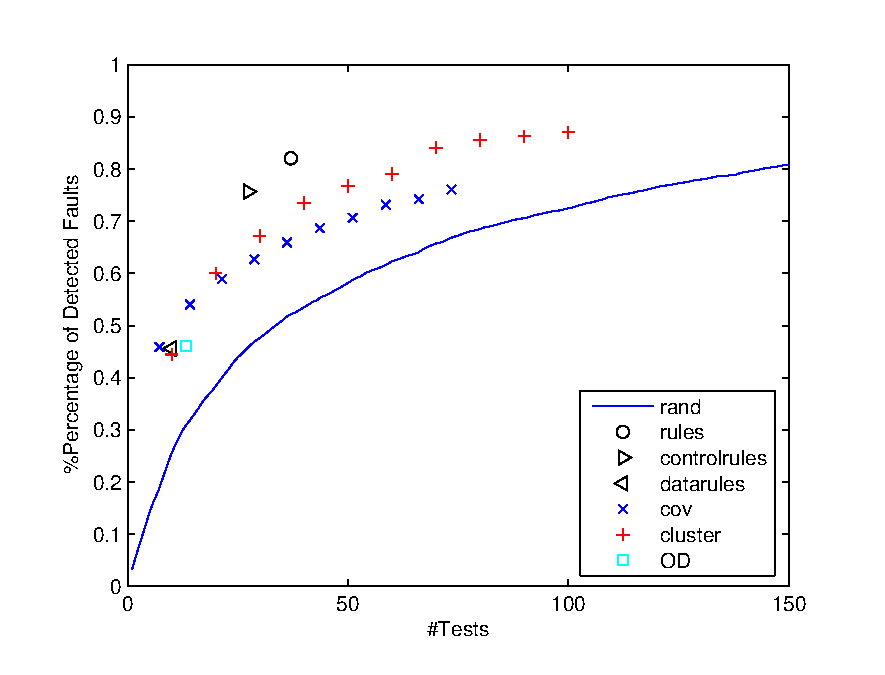
\includegraphics{figs/plotExps_siemens.eps}}
%    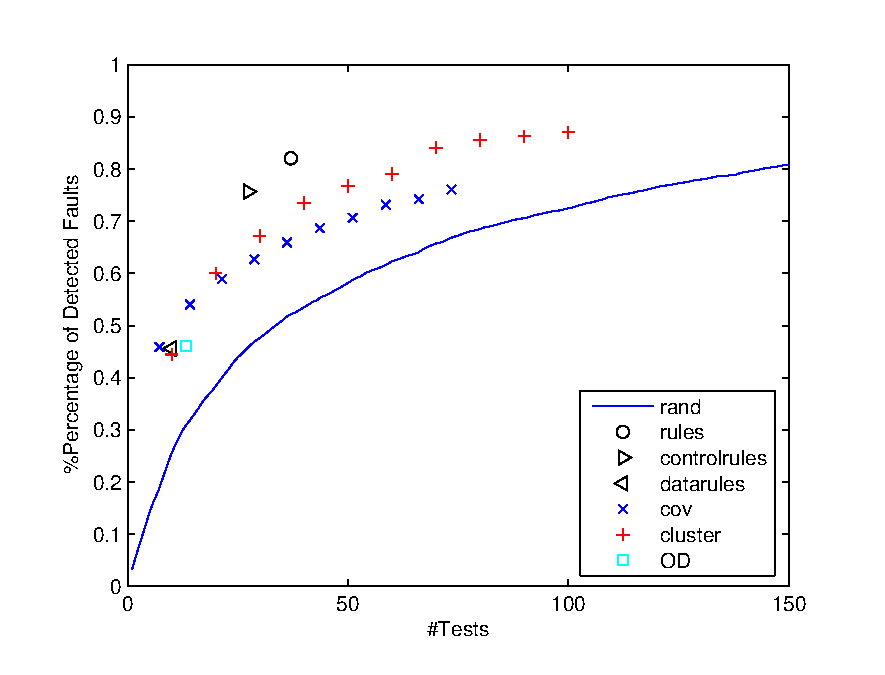
\includegraphics[width=0.35\textwidth]{figs/plotExps_siemens.eps}}
%%  \hspace{0.5in}
%  \subfigure[Results in the space program]{
%    \label{fig:all:b} %% label for second subfigure
%    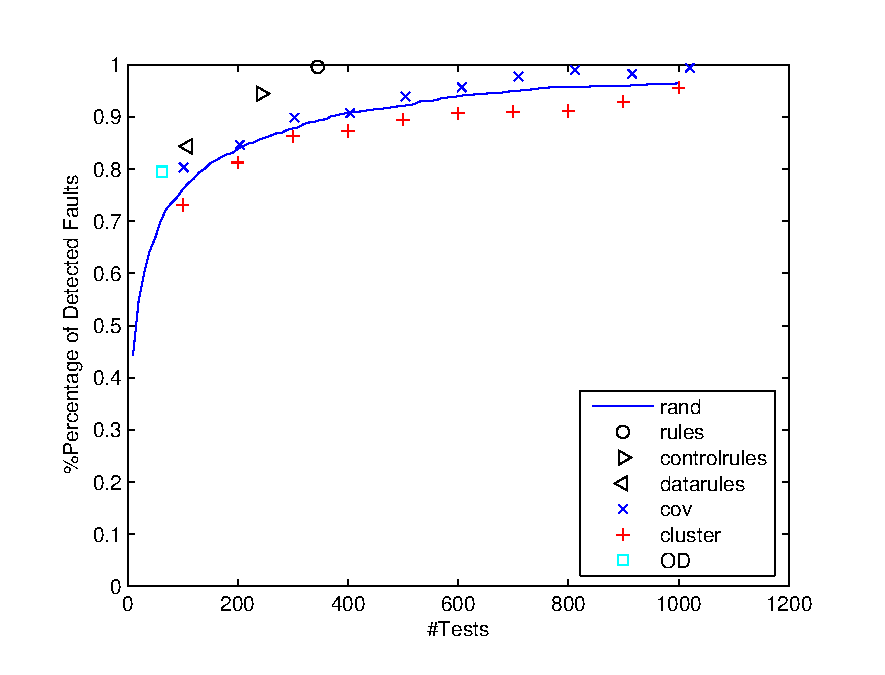
\includegraphics[width=0.35\textwidth]{figs/plotExps_space.eps}}
%  \subfigure[Results in the grep program]{
%    \label{fig:all:c} %% label for second subfigure
%    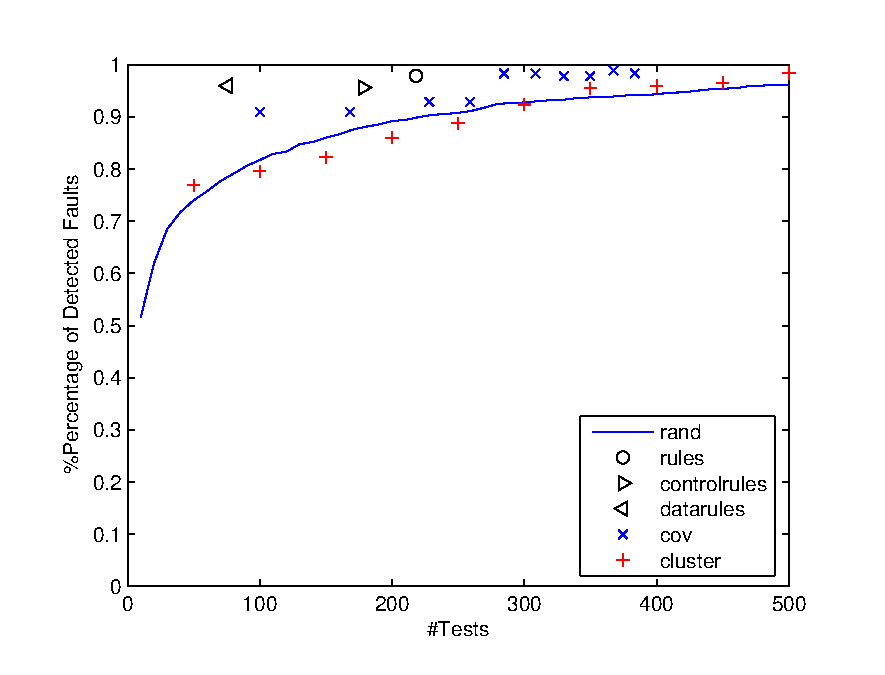
\includegraphics[width=0.35\textwidth]{figs/plotExps_grep.eps}}
%  \caption{Results of all the faults}
%  \label{fig:all} %% label for entire figure
%%\end{figure}
%
%%\begin{figure}
%%  \centering
%  \subfigure[Results in the Siemens program]{
%    \label{fig:nontrivial:a} %% label for first subfigure
%    %\includegraphics{figs/plotExps_diffi_siemens.eps}}
%    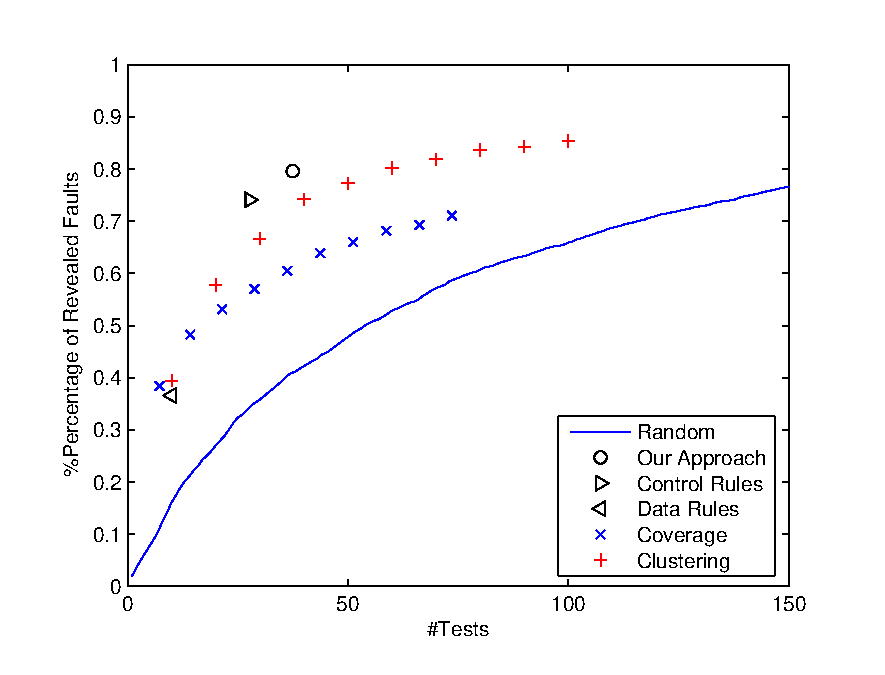
\includegraphics[width=0.35\textwidth]{figs/plotExps_diffi5_siemens.eps}}
%%  \hspace{0.5in}
%  \subfigure[Results in the space program]{
%    \label{fig:nontrivial:b} %% label for second subfigure
%    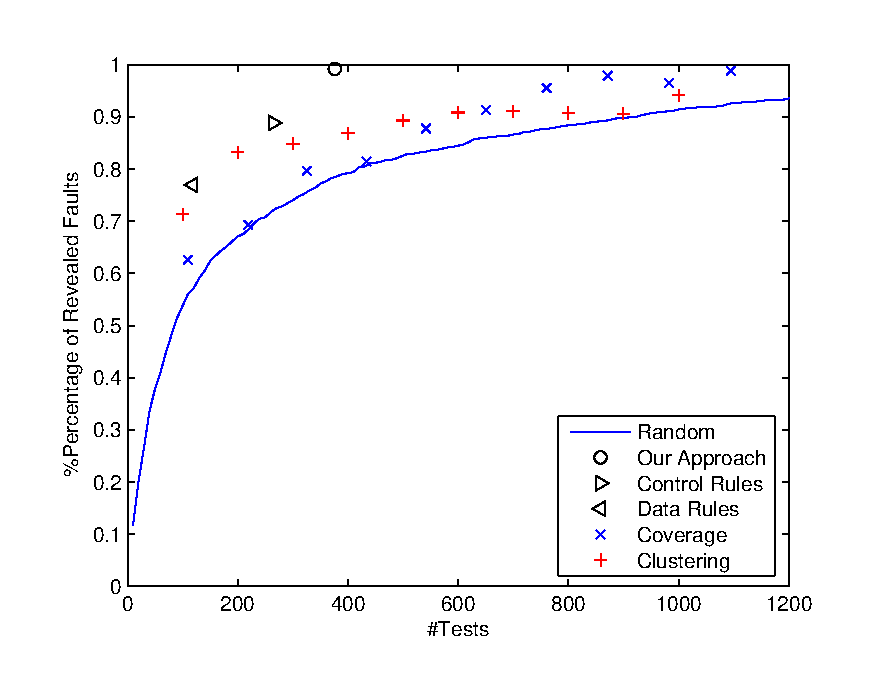
\includegraphics[width=0.35\textwidth]{figs/plotExps_diffi5_space.eps}}
%  \subfigure[Results in the grep program]{
%    \label{fig:nontrivial:c} %% label for second subfigure
%    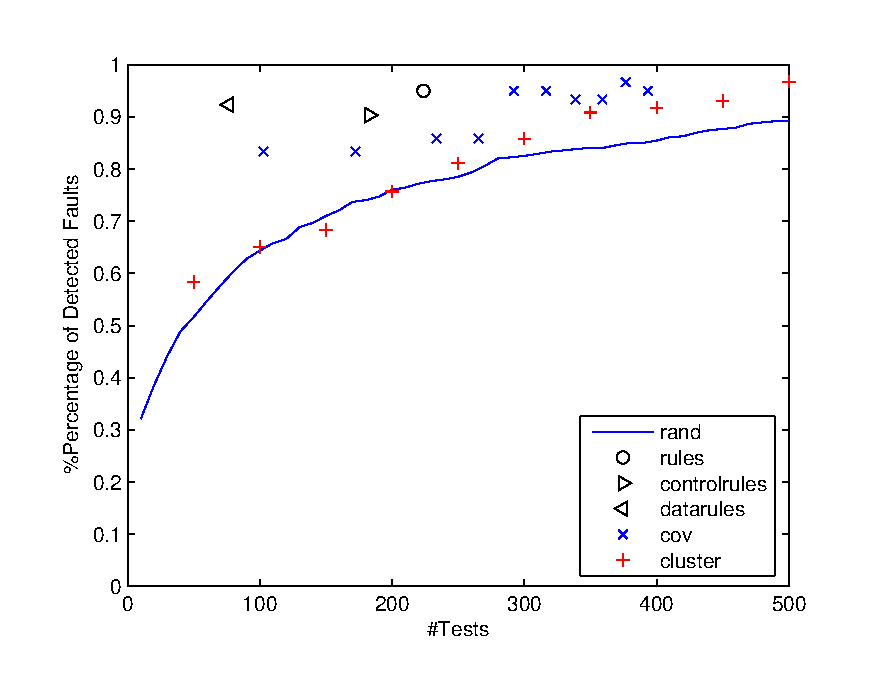
\includegraphics[width=0.35\textwidth]{figs/plotExps_diffi5_grep.eps}}
%  \caption{Results of the nontrivial faults}
%  \label{fig:nontrivial} %% label for entire figure
%\end{figure*}

The first subject is the Siemens suite~\cite{Hutchins94}, which was
created by Siemens researchers. The Siemens researchers created 132
faulty versions of 7 programs that range in size from 170 to 540
lines. The Siemens researchers generated tests automatically from
test-specification scripts, then augmented those tests with
manually-constructed white-box tests such that each exercisable
coverage unit was covered by at least 30 test cases. The numbers of
tests range from 1052 to 5542. There are 130 faults that can be
detected by the test suite in our environment.

The second subject is the {\it Space} program~\cite{Rothermel01},
which interprets Array Definition Language inputs. The {\it Space}
program was developed at the European Space Agency. It has 9564
lines of C code. The test suite of Space contains 13585 test cases,
where 10000 were randomly generated and the remainder were added to
cover every statement or branch at least 30 times. There are 38
faults, among which 34 faults can be detected by the test suite in
our environment.



The third subject is the {\it grep} program, which is a GNU utility
that searches the input files for lines containing a match to a
given pattern list. It has 13358 lines of C code. There are 809 test
cases, which were generated based on informal specifications and
then augmented to increase statement coverage~\cite{SIR}. There are
five original versions of the grep program, each of which was seeded
by a number of faults. In our environment, there are in total 20
faults that can be detected by the test suite.


The characteristic of the subject programs is shown in Table
\ref{tab:subjects}. In these subjects, there are many trivial faults
that fail on more than 5\% of the tests. Such faults are less likely
to be seen in practical setting. To better evaluate the potential
effectiveness of test selection approaches in practice, we conduct
additional experiments on only the nontrivial faults.




\subsection{Measurement}



To evaluate the effectiveness of an approach in test selection, we
use two metrics. The first metric is the size of the selected test
suite, i.e., the number of the selected tests. This metric indicates
the amount of human effort required to check the results of the
selected tests. The second metric is the percentage of faults that
can be detected by the selected tests. A set of tests are said to
detect a fault if the faulty program fails on one or more of the
tests. We would like to reveal as many faults as possible. A good
test-selection algorithm should select a small number of tests that
can reveal most of the faults.



\subsection{Results}



Figures \ref{fig:all} and \ref{fig:nontrivial} show the results of
our approach and the existing test selection approaches, including
the code-coverage-based, clustering-based, and
dynamic-invariant-based approaches. The x-axis is the number of
selected tests and the y-axis is the percentage of faults revealed
by the selected tests. We also present the results of random
selection as the comparison baseline. Because the three subjects are
quite different in the program size and the original test suite
size, we present the results in these three subjects separately.
Tables \ref{tab:our}, \ref{tab:other}, \ref{tab:our:nontrivial}, and
\ref{tab:other:nontrivial} show some of the detailed results,
including the number of selected tests and the percentage of
revealed faults in each subject program. To reduce the potential
effect of random noise, we run all of the experiments 50 times and
then report the averaged results.



\subsubsection{Effectiveness of Our Approach}



\begin{figure}
%  \centering
  \subfigure[Results in the Siemens program]{
    \label{fig:all:a} %% label for first subfigure
    %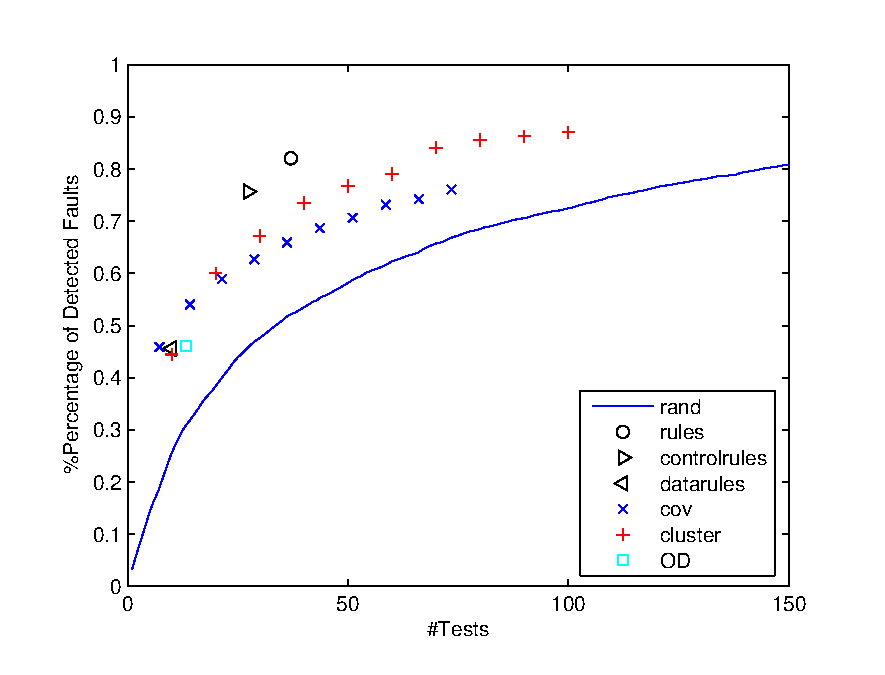
\includegraphics{figs/plotExps_siemens.eps}}
    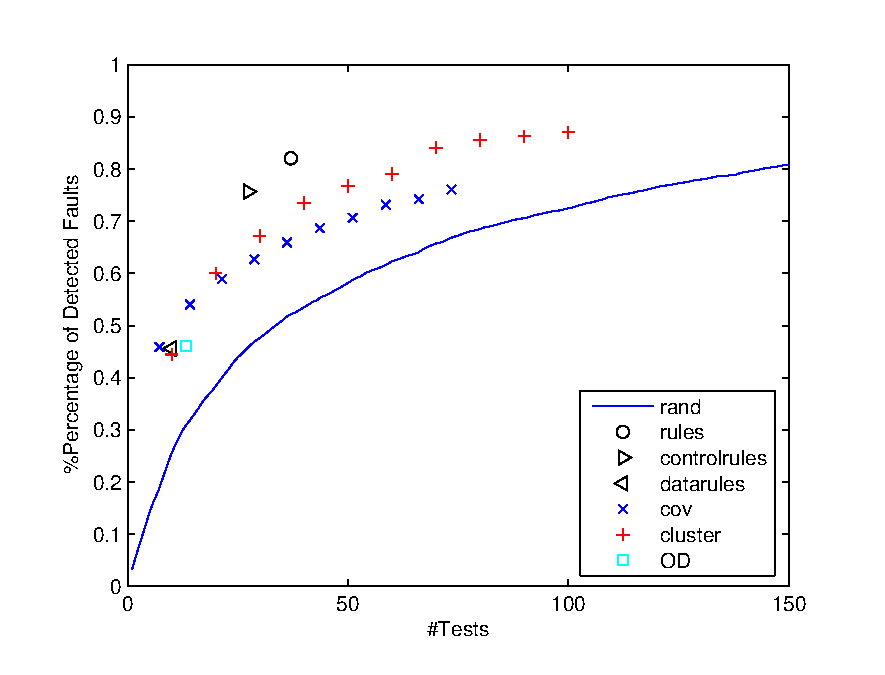
\includegraphics[width=0.5\textwidth]{figs/plotExps_siemens.eps}}
%  \hspace{0.5in}
  \subfigure[Results in the space program]{
    \label{fig:all:b} %% label for second subfigure
    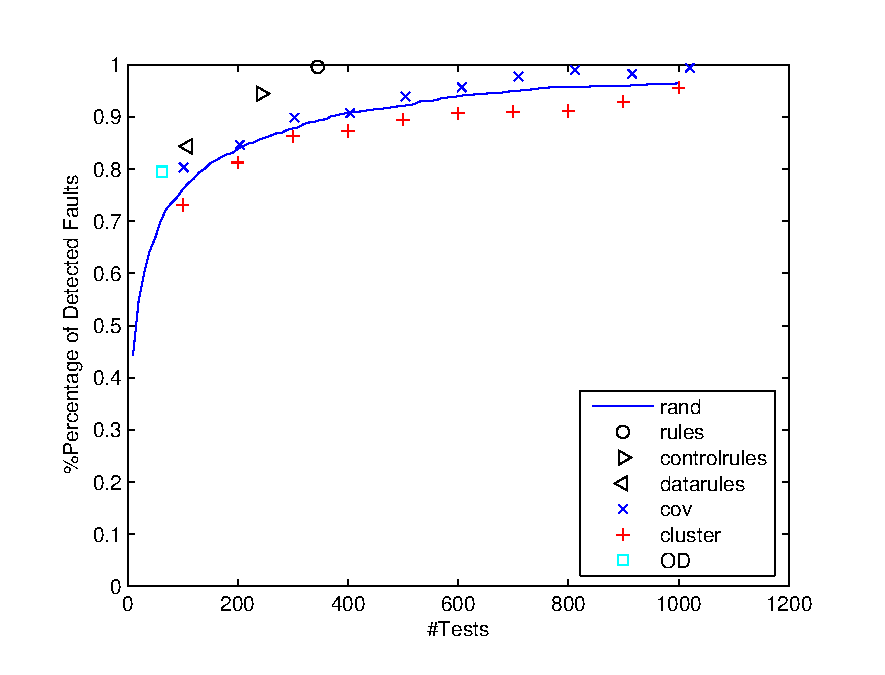
\includegraphics[width=0.5\textwidth]{figs/plotExps_space.eps}}
  \subfigure[Results in the grep program]{
    \label{fig:all:c} %% label for second subfigure
    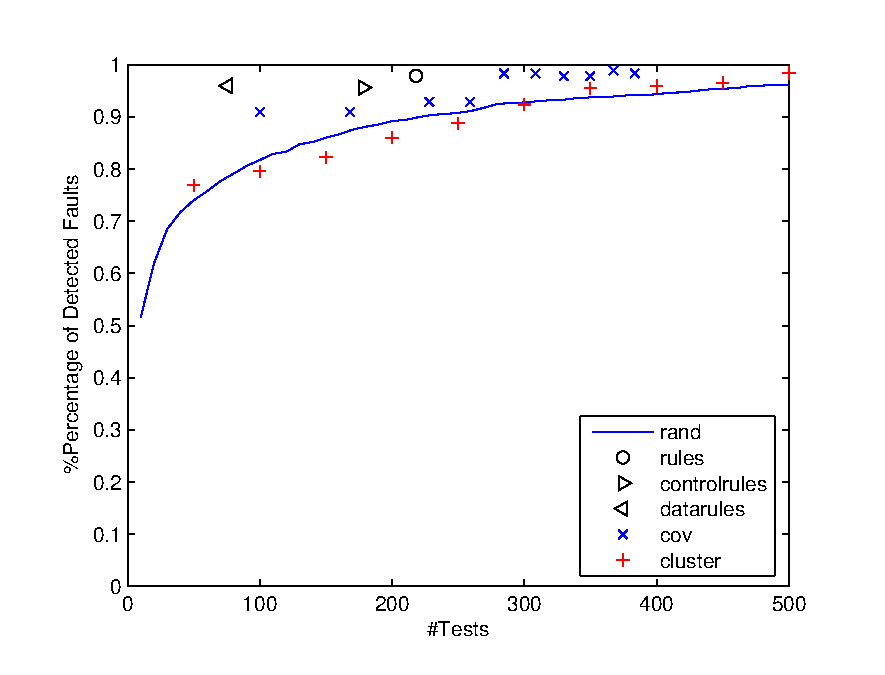
\includegraphics[width=0.5\textwidth]{figs/plotExps_grep.eps}}
  \caption{Results of all the faults}
  \label{fig:all} %% label for entire figure
\end{figure}

\begin{figure}
%  \centering
  \subfigure[Results in the Siemens program]{
    \label{fig:nontrivial:a} %% label for first subfigure
    %\includegraphics{figs/plotExps_diffi_siemens.eps}}
    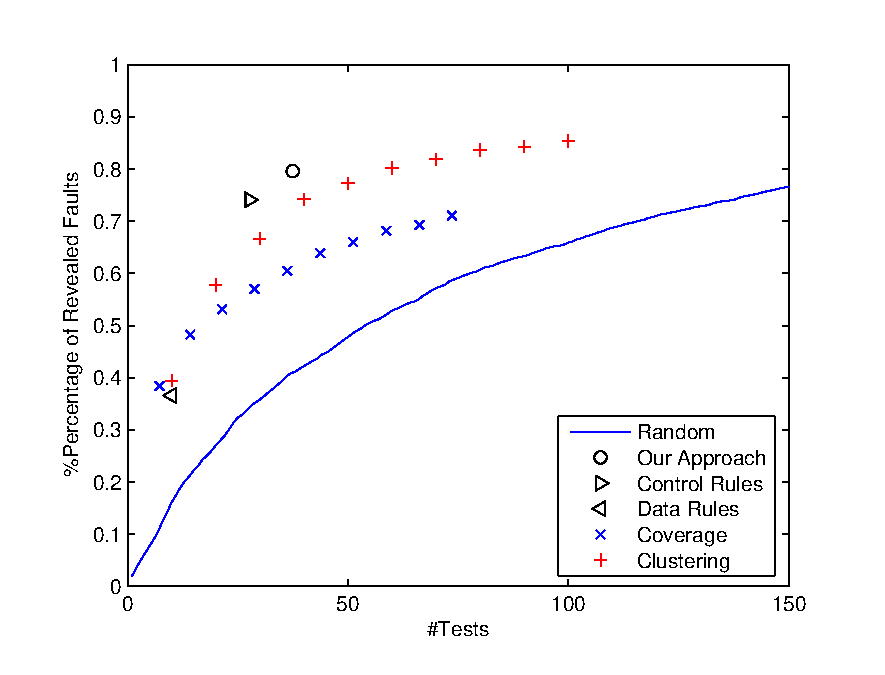
\includegraphics[width=0.5\textwidth]{figs/plotExps_diffi5_siemens.eps}}
%  \hspace{0.5in}
  \subfigure[Results in the space program]{
    \label{fig:nontrivial:b} %% label for second subfigure
    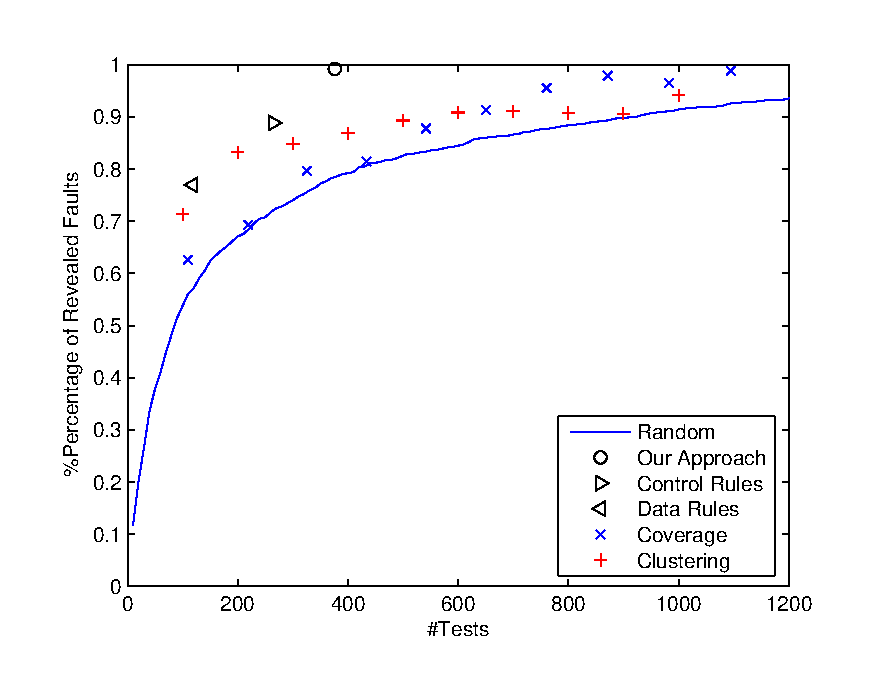
\includegraphics[width=0.5\textwidth]{figs/plotExps_diffi5_space.eps}}
  \subfigure[Results in the grep program]{
    \label{fig:nontrivial:c} %% label for second subfigure
    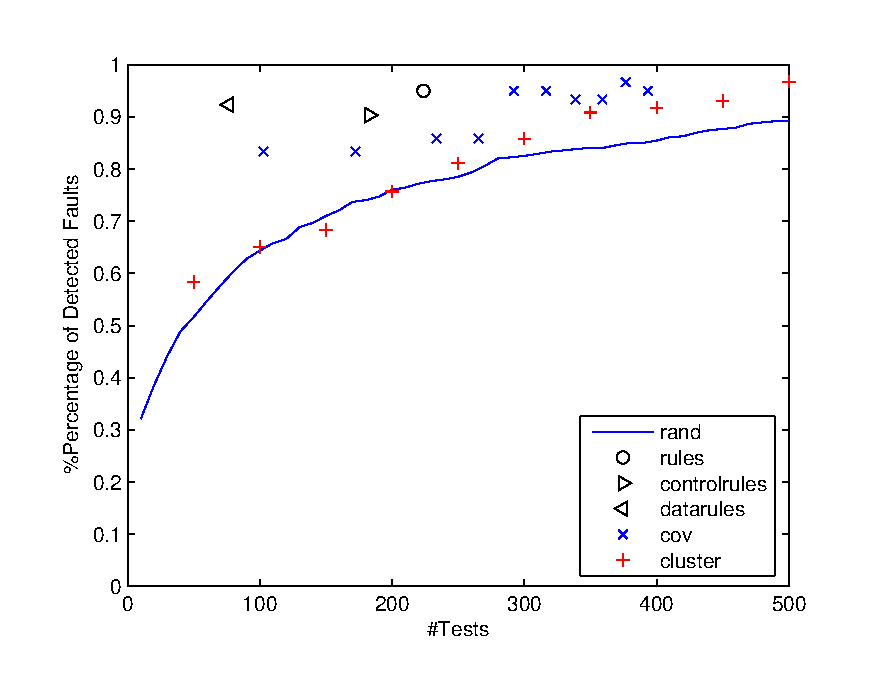
\includegraphics[width=0.5\textwidth]{figs/plotExps_diffi5_grep.eps}}
  \caption{Results of the nontrivial faults}
  \label{fig:nontrivial} %% label for entire figure
\end{figure}




%\begin{figure*}
%  \centering
%  \hspace{-0.2in}
%  \subfigure[Results in the Siemens program]{
%    \label{fig:all:a} %% label for first subfigure
%    %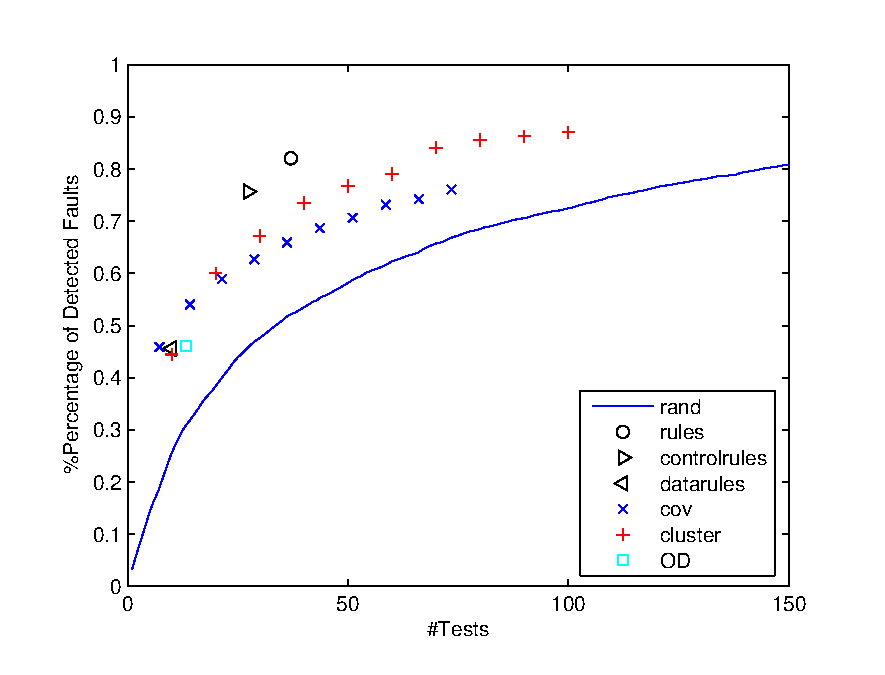
\includegraphics{figs/plotExps_siemens.eps}}
%    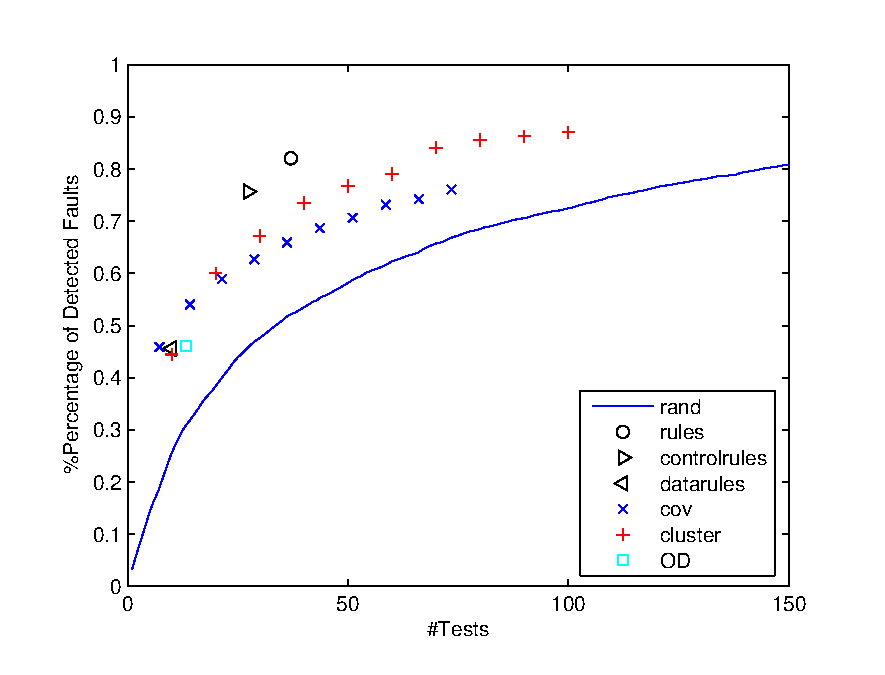
\includegraphics[width=0.35\textwidth]{figs/plotExps_siemens.eps}}
%  \hspace{-0.4in}
%  \subfigure[Results in the space program]{
%    \label{fig:all:b} %% label for second subfigure
%    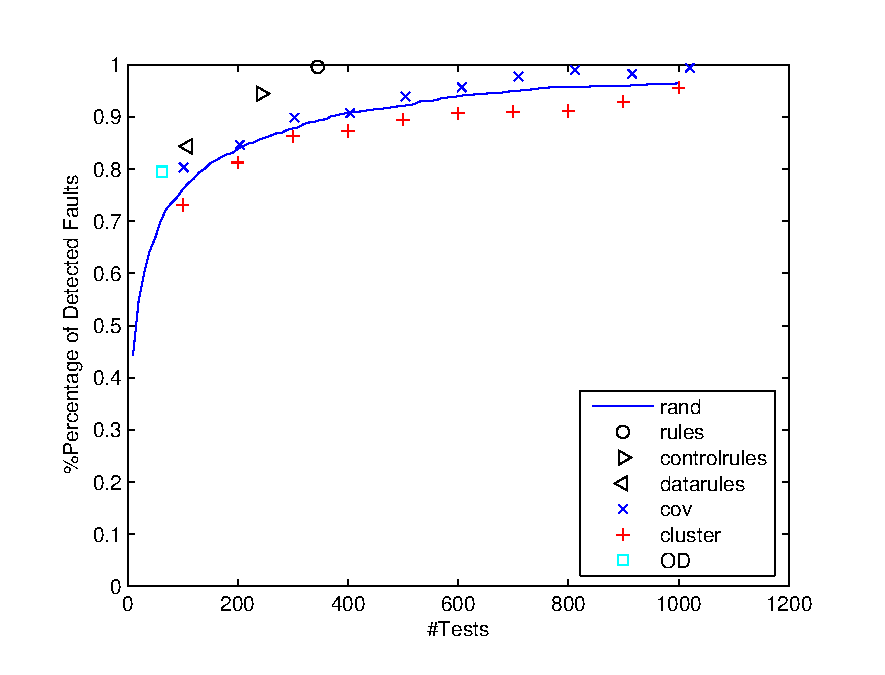
\includegraphics[width=0.35\textwidth]{figs/plotExps_space.eps}}
%  \hspace{-0.4in}
%  \subfigure[Results in the grep program]{
%    \label{fig:all:c} %% label for second subfigure
%    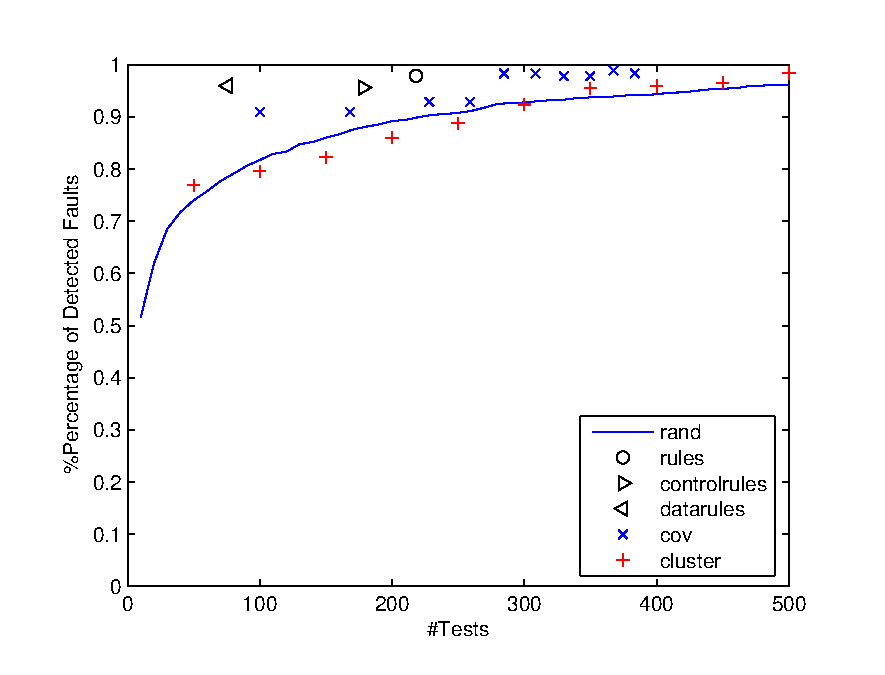
\includegraphics[width=0.35\textwidth]{figs/plotExps_grep.eps}}
%  \hspace{-0.2in}
%  \caption{Results of all the faults}
%  \label{fig:all} %% label for entire figure
%\end{figure*}

\begin{table*}[htbp]
\caption{Results of our approach on all the faults}\label{tab:our}
\center
\begin{tabular}{|c|c|c|c|c|c|c|c|c|}
\hline Program   & \multicolumn{2}{c}{Original Test Suite} \vline & \multicolumn{2}{c}{Our Approach} \vline
& \multicolumn{2}{c}{Control Rules} \vline & \multicolumn{2}{c}{Data Rules} \vline   \\

\cline{2-9}   & \#Tests &   \%Faults & \#Tests &   \%Faults &
\#Tests &   \%Faults & \#Tests &   \%Faults \\
\hline  print\_tokens   &   4130    &   100 &   25  &   89  &   17  &   88  &   8   &   50  \\
\hline  print\_tokens2  &   4115    &   100 &   41  &   100 &   30  &   100 &   10  &   61  \\
\hline  replace &   5542    &   100 &   75  &   80  &   60  &   73  &   16  &   37  \\
\hline  schedule    &   2650    &   100 &   31  &   86  &   24  &   70  &   7   &   49  \\
\hline  schedule2   &   2710    &   100 &   32  &   62  &   24  &   61  &   9   &   25  \\
\hline  tcas    &   1608    &   100 &   26  &   74  &   15  &   68  &   12  &   23  \\
\hline  tot\_info &   1052    &   100 &   29  &   84  &   21  &   71  &   9   &   74  \\
\hline  Siemens suite   &   3115    &   100 &   \textbf{37}  &   \textbf{82}  &   27  &   76  &   10  &   46  \\
\hline  Space   &   13585   &   100 &   \textbf{345} &   \textbf{100} &   242 &   94  &   109 &   84  \\
%\hline  grep    &   809 &   100 &   219 &   97  &   178 &   94  &   76  &   95  \\
\hline  grep    &   809 &   100 &   \textbf{218} &   \textbf{98}  &   178 &   96  &   75  &   96  \\

\hline
\end{tabular}
\end{table*}

\begin{table*}[htbp]
\caption{Results of other approaches on all the
faults}\label{tab:other} \center
\begin{tabular}{|c|c|c|c|c|c|c|c|c|c|c|}
%\hline Program   & \multicolumn{2}{c}{Original Test Set} \vline & \multicolumn{3}{c}{Covering Branches} \vline  \\

\hline Program   & \multicolumn{2}{c}{Original } \vline &
\multicolumn{2}{c}{Random} \vline &
\multicolumn{2}{c}{Code-coverage-based} \vline &
\multicolumn{2}{c}{Clustering-based} \vline &
\multicolumn{2}{c}{Operational} \vline
    \\

& \multicolumn{2}{c}{Test Suite} \vline &
\multicolumn{2}{c}{Selection} \vline & \multicolumn{2}{c}{Approach
(k=1)} \vline & \multicolumn{2}{c}{Approach} \vline &
\multicolumn{2}{c}{Difference} \vline
   \\

 \cline{2-11}  & \#Tests &   \%Faults & \#Tests &   \%Faults &
\#Tests &   \%Faults & \#Tests &   \%Faults & \#Tests &   \%Faults  \\


\hline  print\_tokens   &   4130    &   100 &   37  &   39&   6   &   61  &   40  &   84  &   9   &   37   \\
\hline  print\_tokens2  &   4115    &   100 &   37  &   78&   4   &   90  &   40  &   100 &   6   &   51    \\
\hline  replace &   5542    &   100 &   37  &   45&   12  &   33  &   40  &   57  &   18  &   45    \\
\hline  schedule    &   2650    &   100 &   37  &   48&   7   &   26  &   40  &   60  &   10  &   33   \\
\hline  schedule2   &   2710    &   100 &   37  &   34&   5   &   26  &   40  &   47  &   13  &   30    \\
\hline  tcas    &   1608    &   100 &   37  &   46&   11  &   31  &   40  &   84  &   26  &   55    \\
\hline  tot\_info &   1052    &   100 &   37  &   75&   5   &   53  &   40  &   82  &   9   &   72   \\
\hline  Siemens suite   &   3115    &   100 &   \textbf{37}  &   \textbf{52}&   \textbf{7}   &   \textbf{46}  &   \textbf{40}  &   \textbf{73}  &   \textbf{13}  &   \textbf{46}   \\
\hline  Space   &   13585   &   100 &   \textbf{345} &   \textbf{89}&   \textbf{102} &   \textbf{80}  &   \textbf{400} &   \textbf{87}  &   \textbf{63}  &   \textbf{80}  \\
%\hline  grep    &   809 &   100 &   101 &   90  &   250 &   91  &   -   &   -     \\
\hline  grep    &   809 &   100 &   \textbf{219} &   \textbf{90}&   \textbf{100} &   \textbf{91}  &   \textbf{250} &   \textbf{89}  &   -   &   -     \\

\hline
\end{tabular}
\end{table*}


\begin{table*}[htbp]
\caption{Results of our approach on nontrivial
faults}\label{tab:our:nontrivial} \center
\begin{tabular}{|c|c|c|c|c|c|c|c|c|}

\hline Program   & \multicolumn{2}{c}{Original Test Suite} \vline &
\multicolumn{2}{c}{Our Approach} \vline
& \multicolumn{2}{c}{Control Rules} \vline & \multicolumn{2}{c}{Data Rules} \vline   \\

\cline{2-9}  & \#Tests &   \%Faults & \#Tests &   \%Faults &
\#Tests &   \%Faults & \#Tests &   \%Faults \\
\hline  print\_tokens   &   4130    &   100 &   25  &   89  &   17  &   88  &   8   &   50  \\
\hline  print\_tokens2  &   4115    &   100 &   42  &   100 &   32  &   100 &   10  &   38  \\
\hline  replace &   5542    &   100 &   75  &   78  &   60  &   71  &   16  &   35  \\
\hline  schedule    &   2650    &   100 &   32  &   87  &   25  &   84  &   7   &   35  \\
\hline  schedule2   &   2710    &   100 &   32  &   62  &   24  &   61  &   9   &   25  \\
\hline  tcas    &   1608    &   100 &   26  &   72  &   15  &   65  &   12  &   18  \\
\hline  tot\_info &   1052    &   100 &   30  &   69  &   21  &   50  &   9   &   55  \\
\hline  Siemens suite   &   3115    &   100 &   \textbf{37}  &   \textbf{80}  &   28  &   74  &   10  &   37  \\
\hline  Space   &   13585   &   100 &   \textbf{376} &   \textbf{99}  &   265 &   89  &   118 &   77  \\
%\hline  grep    &   809 &   100 &   225 &   93  &   184 &   87  &   77  &   90  \\
\hline  grep    &   809 &   100 &   \textbf{224} &   \textbf{95}  &   183 &   90  &   76  &   92  \\

\hline
\end{tabular}
\end{table*}

\begin{table*}[htbp]
\caption{Results of other approaches on nontrivial
faults}\label{tab:other:nontrivial} \center
\begin{tabular}{|c|c|c|c|c|c|c|c|c|}

\hline Program   & \multicolumn{2}{c}{Original } \vline &
\multicolumn{2}{c}{Random} \vline &
\multicolumn{2}{c}{Code-coverage-based} \vline &
\multicolumn{2}{c}{Clustering-based} \vline     \\

& \multicolumn{2}{c}{Test Suite} \vline &
\multicolumn{2}{c}{Selection} \vline & \multicolumn{2}{c}{Approach
(k=1)} \vline &
\multicolumn{2}{c}{Approach} \vline     \\

 \cline{2-9}  & \#Tests &   \%Faults & \#Tests &   \%Faults &
\#Tests &   \%Faults & \#Tests &   \%Faults \\


\hline  print\_tokens   &   4130    &   100 &   37  &   39&   6   &   61  &   40  &   84  \\
\hline  print\_tokens2  &   4115    &   100 &   37  &   54&   5   &   76  &   40  &   100 \\
\hline  replace &   5542    &   100 &   37  &   42&   12  &   32  &   40  &   60  \\
\hline  schedule    &   2650    &   100 &   37  &   26&   7   &   26  &   40  &   80  \\
\hline  schedule2   &   2710    &   100 &   37  &   34&   5   &   26  &   40  &   47  \\
\hline  tcas    &   1608    &   100 &   37  &   40&   11  &   25  &   40  &   82  \\
\hline  tot\_info &   1052    &   100 &   37  &   51&   5   &   23  &   40  &   67  \\
\hline  Siemens suite   &   3115    &   100 &   \textbf{37}  &   \textbf{41}&   \textbf{7}   &   \textbf{38}  &   \textbf{40}  &   \textbf{74}  \\
\hline  Space   &   13585   &   100 &   \textbf{376} &   \textbf{79}&   \textbf{110} &   \textbf{63}  &   \textbf{400} &   \textbf{87}  \\
%\hline  grep    &   809 &   100 &   103 &   78  &   250 &   79  \\
\hline  grep    &   809 &   100 &   \textbf{225} &   \textbf{77}&   \textbf{103} &   \textbf{83}  &   \textbf{250} &   \textbf{81}  \\

\hline
\end{tabular}
\end{table*}



We observe that our approach is effective in reducing the number of
tests while revealing most of the faults. In the Siemens suite (all
faults), our approach selects only 37 tests for the programs on
average, which can still reveal 82\% of the faults. In the space and
the grep programs (all faults), our approach selects 345 and 219
tests on average, which can reveal 100\% and 97\% of the faults,
respectively. We note that randomly selecting the same number of
tests as our approach can also reveal 52\%, 89\% and 90\% of the
faults in these subjects. This result is due to two main factors:
(1) many trivial faults can be easily revealed and (2) the
probability of finding no failures of a fault decreases
exponentially with the number of selected tests. Checking the
results in nontrivial faults, we can see that our approach is still
effective while the effectiveness of random selection decreases
much. For example, in the Siemens suite (nontrivial faults), our
approach selects only 37 tests for the programs on average, which
can still reveal 80\% of the faults. Randomly selecting the same
number of tests can reveal only 41\% of the faults.

We also evaluate the effects of the two kinds of common operational
models that we proposed, i.e., control rules and data rules,
separately. The results are plotted in Figures \ref{fig:all} and
\ref{fig:nontrivial}, and shown in Tables \ref{tab:our} and
\ref{tab:our:nontrivial}. We observe that both these two kinds of
rules are helpful in revealing faults. Among them, covering
violations of control rules can detect more faults than covering
violations of data rules, but also requires much more tests. The
data rules are better for some programs such as tot\_info, which is
an information measure program that deals with data tables. In
summary, these two kinds of rules are complementary to each other as
they reflect different aspects of program behaviors. When combined
together, they are able to help select quite a good subset of tests.




\subsubsection{Comparison with the Code-coverage-based Approach}

We compare our approach with the code-coverage-based approach. The
code-coverage-based approach attempts to cover as many program
elements of a given type as the original test suite with as few test
cases as possible~\cite{Leon05}. Selecting a minimal-size,
coverage-maximizing subset of a test suite is an instance of the
set-cover problem, which is often solved using a greedy
approximation algorithm. On each of its iterations, the greedy
algorithm selects the test that covers the largest number of
elements not covered by the previously selected tests. This approach
is based on the assumption that many software faults and their
caused failures can be revealed simply by exercising such elements,
regardless of other factors. To evaluate the potential capability of
finding more faults using the code-coverage-based approach, we also
extend the basic code-coverage-based approach by increasing the
number of times each program element should be covered. We say a
program element is covered k times if there are k different tests
that cover it. We use the branch coverage and we experiment with k
from 1 to 10. The results are plotted in Figures \ref{fig:all} and
\ref{fig:nontrivial}, and shown in Tables \ref{tab:other} and
\ref{tab:other:nontrivial}.

We observe that the basic code-coverage-based approach, in which
each branch is covered at least once, is good in selecting a small
subset of tests that can reveal many faults. However, it misses many
other faults, e.g., it misses more than half of the faults in the
Siemens suite. Our approach can select a test suite with a much
higher fault-revealing capability, and the number of selected tests
is only a few times larger than that of the basic
code-coverage-based approach. Increasing the number of the times
that each branch should be covered helps reveal more faults, but is
less cost-effective than our approach. Sometimes increasing k may
decrease the percentage of revealed faults. Such an observation is
due to that the smallest subset of tests that covers each program
element at least k times may not be a subset of the smallest subset
of tests that covers each program element at least k+1 times.



\subsubsection{Comparison with the Clustering-based Approach}

We next compare the results of our approach with the results of the
clustering-based approach~\cite{Dickinson01a}. The clustering-based
approach uses agglomerative hierarchical clustering to cluster the
tests, and then selects one test from each cluster. The main
assumption of the clustering-based approach is that a significant
number of failures are isolated in clusters of small size. Besides
one-per-cluster sampling, there are other possible sampling schemes
that aim at finding more failing tests for each
fault~\cite{Dickinson01b}. As our concern is to increase the
likelihood of finding at least one failing test for each fault, we
do not compare our approach with these other sampling schemes. We
use the binary branch profiles for clustering. We do not use the
variable-value profiles since a variable may not be observed in all
the tests. We experiment with 10 different values of the number of
the clusters. The values are 10 to 100, 100 to 1000, and 50 to 500
in the Siemens suite, the space program, and the grep program,
respectively. We select these values based on the program sizes and
the numbers of tests selected by the code-coverage-based approach.
The results are plotted in Figures \ref{fig:all} and
\ref{fig:nontrivial}, and shown in Tables \ref{tab:other} and
\ref{tab:other:nontrivial}.

We observe that the clustering-based approach performs better than
random selection in the Siemens suite (all faults), the Siemens
suite (nontrivial faults), and the space program (nontrivial
faults), but not better than random selection in the other
experiments. There are two main reasons for such results. First,
there is a large number of tests in the Siemens and the space
program. The tests could be highly redundant, especially for the
common execution paths. The clustering-based approach may then help
to cover more different execution paths. However, there are not a
large number of tests in the grep program, and these tests are not
redundant. In this case, the clustering-based approach may not help
cover more different execution paths or isolate the most suspicious
tests. Second, there are many trivial faults in the space program
and the grep program, which may violate the assumption of the
clustering-based approach that a significant number of failures are
isolated in clusters of small size. Our approach can isolate tests
that are suspicious in some program elements. It is more stable in
different cases and is better than the clustering-based approach in
general.



\subsubsection{Comparison with the Dynamic-Invariant-based Approach}

Finally, we compare our approach with the dynamic-invariant-based
approach. Harder et al. \cite{Harder03} proposed the operational
difference approach to select tests based on Daikon. It starts with
an empty test suite and repeatedly adds new tests if they violate
the invariants of the previously selected tests. To control the
number of tests, the algorithm terminates when n (n=50 in their
experiments) consecutive tests are considered and rejected. They
also conducted experiments on the Siemens suite and the space
program that we used. We adopt the experimental results from their
original paper directly, which are shown in Table \ref{tab:other}
and plotted in Figure \ref{fig:all}. No result of the operational
difference approach in the grep program or on the nontrivial faults
is available (Daikon cannot be scalable to deal with the grep
program and therefore poses barriers for us to re-implement and
apply the operational difference approach on the grep program).



We observe that the operational difference approach performs
similarly to the basic code-coverage-based approach. It works well
in selecting a small subset of tests that can reveal many faults.
However, it misses many other faults at the same time. The
operational difference approach may be able to reveal more faults if
the termination condition is removed. However, it may then select
much more tests due to the false positives in the detected
invariants. By using the information of all the unverified tests at
hand, our approach can reduce the noise of mined operational models
and thus select a reasonably sized subset of tests that can reveal
most of the faults.





\subsubsection{Efficiency}



To evaluate the efficiency of our approach, we measure the time cost
of our approach on the three subjects, compared with that of the
basic code-coverage-based approach and that of the clustering-based
approach. The result is shown in Table \ref{tab:effi}.

\begin{table}[t]
\caption{Efficiency of Our Approach
(\emph{seconds})}\label{tab:effi} \center
\begin{tabular}{|c|c|c|c|c|c|}
\hline Program   & LOC \hspace{-0.3cm}& \hspace{-0.2cm}\#Tests\hspace{-0.1cm} & Our  & \hspace{-0.1cm}Coverage\hspace{-0.1cm} & \hspace{-0.1cm}Clustering\hspace{-0.1cm}   \\
& & & \hspace{-0.1cm}\footnotesize{Approach}\hspace{-0.1cm} &  &  \\

\hline  print\_tokens   &   539 &   4130    &   1.4 &   0.4 &   366.2   \\
\hline  print\_tokens2  &   489 &   4115    &   5.4 &   0.7 &   82.5    \\
\hline  replace &   507 &   5542    &   7.8 &   1.0 &   390 \\
\hline  schedule    &   397 &   2650    &   1.0 &   0.2 &   65.1    \\
\hline  schedule2   &   299 &   2710    &   1.3 &   0.2 &   93.8    \\
\hline  tcas    &   174 &   1608    &   0.7 &   0.1 &   38.8    \\
\hline  tot\_info   &   398 &   1052    &   0.8 &   0.1 &   14.7    \\
\hline  \hspace{-0.1cm}Siemens suite\hspace{-0.1cm}   &   400 &   3115    &   2.6 &   0.4 &   150.2   \\
\hline  Space   &   9564    &   13585   &   598.8   &   5.4 &   1364    \\
\hline  grep    &   \hspace{-0.1cm}13358 \hspace{-0.1cm}  &   809 &   92.9    &   4.9 &   6.8 \\


\hline
\end{tabular} \vspace{-0.2in}
\end{table}

Among the three approaches, the basic code-coverage-based approach
is the fastest. It takes at most a few seconds in each of the
subject programs. The clustering-based approach is fast in the grep
program but is not fast in other programs. Basically, the more tests
there are, the longer time the clustering-based approach takes.
However, there is no clear polynomial relationships between the time
cost and the number of tests. The time cost of the clustering
approach can be greatly affected by the distribution of the tests.
Our approach is fast in the Siemens suite and takes reasonable time
in the space program and the grep program. More specifically, our
approach takes about 10 minutes in the space program, which contains
about 9564 lines of code and 13,585 tests. However, our approach may
not be efficient enough for large programs with large test suites.
The main cost of our approach is the time of mining the control
rules, which is proportional to the number of tests and to the
square of the number of branches. For a large program with 100,000
lines of code and a large test suite that has 13,585 tests, our
approach may take about 20 hours. In this case, a possible
improvement is to mine only the control rules between the branches
in the same modules. We can then greatly reduce the number of
candidate control rules and thus the time cost of our approach.

\vspace{-0.1in}
\subsubsection{Summary and Discussions}

Our results suggest the following observations:

\begin{itemize}
\item \vspace{-0.1in}
Our approach is effective in reducing the number of tests while
revealing most of the faults. Control rules and data rules are
complementary to each other as they reflect different aspects of
program behaviors.


\item \vspace{-0.1in}
Our approach can select a test suite with a much higher
fault-revealing capability than those of the code-coverage-based
approach and the dynamic-invariant-based approach, and is more
robust and cost-effective than the clustering-based approach.
%However, we have not compared the effectiveness of our approach with
%that of maximizing more complex coverage profiles, which are more
%difficult to collect. The clustering approach is more flexible for
%selecting different numbers of tests. Finally, the dynamic
%invariants are useful for multiple purposes besides test selection.
But we note that there are some issues to be considered. The
code-coverage-based approach may reveal more faults if more complex
coverage profiles are used, which however are more difficult to
collect. The clustering approach is more flexible for selecting
different numbers of tests.
\item \vspace{-0.1in}
Our approach takes reasonable time for small to medium sized
programs with large test suites. However, it may not be efficient
enough for large programs with large test suites. This issue may be
alleviated by mining only the control rules between the branches in
the same modules. We need to conduct further experiments to
investigate this technique.
\end{itemize}
%Our current experiments are based on existing test suites whose
%tests are manually or randomly generated. In automated testing, a
%number of test generation approaches generate tests systematically.
%It is valuable for our future work to investigate how our approach
%can work on the test sets automatically generated by these
%approaches.

\subsection{Threats to Validity}
The threats to external validity primarily include the degree to
which the subject programs, faults, and test cases are
representative of true practice. The Siemens programs are small and
the space program is of medium size. Most of the faulty versions
involve simple, one or two-line manually seeded faults. Moreover,
the tests are manually or randomly generated, while in automated
testing, a number of test generation approaches generate tests
systematically. These threats could be reduced by more experiments
on wider types of subjects with systematically generated tests in
future work. The threats to internal validity include the fact that
different approaches select different numbers of tests. This fact
may make the comparison of fault-revealing effectiveness bias to the
approaches that select larger number of tests. To reduce this bias,
we present the results of random selection as the baseline. We also
try to evaluate the fault-revealing capabilities of other approaches
with different numbers of selected tests.



%-------------------------------------------------------------------------
\section{Related Work} \label{sec:relatedwork}

In this section, we describe existing work in test selection, which
can be classified into five main categories.



\textbf{Black-box Test Selection.} There exist a number of
black-box approaches for test selection. In partition
testing~\cite{Myers79}, a test input domain is divided into
subdomains based on some criteria, and then developers can select
one or more representative inputs from each subdomain. Our approach
partitions the tests based on mining common software behaviors,
without requiring any knowledge of input domains. When \emph{a
priori} specifications are provided for a program, Chang and
Richardson \cite{Chang99} used specification coverage criteria to
select a candidate set of test cases that exercise new aspects of
the specification. Our approach does not require \emph{a priori}
specifications.

% model coverage

\textbf{Code-coverage-based Test Selection.} Various kinds of code
coverage criteria have been proposed for test selection, such as
control-flow testing criteria~\cite{Huang75} and data-flow testing
criteria \cite{Frankl88}. Hutchins et al. \cite{Hutchins94} reported
an experimental study investigating the effectiveness of
control-flow and data-flow testing criteria. Their results suggested
that test sets achieving high code coverage levels usually showed
significantly better fault-detection capability than randomly chosen
test sets of the same size. However, the results also indicated that
100\% code coverage alone is not a reliable indicator of the
effectiveness of a test set. Leon et al. \cite{Leon05} evaluated the
effectiveness of complex information flow criteria, which model
indirect control/data dependencies between instructions or objects,
for test selection. Their results suggested that test sets
maximizing complex information flow criteria revealed more faults
than test sets maximizing block coverage with substantial additional
cost, and in some subjects the profiles could not be generated due
to memory constraints. Our approach is based on low overhead
profiles, such as branch coverage and data value bounds. Yet our
approach can reveal most of the faults by mining and violating
implication relationships between branches and constraints of data
values.

\textbf{Clustering-based Test Selection.} Dickinson et
al.~\cite{Dickinson01a} used clustering analysis to partition
executions based on structural profiles, and employed sampling
techniques to select executions from clusters for result inspection.
They further proposed a failure-pursuit sampling approach
\cite{Dickinson01b} to enhance the efficiency in finding failures.
Moreover, Leon et al. \cite{Leon05} evaluated the effectiveness of
clustering analysis based on complex information flow criteria.
Their results suggested that the effectiveness of the clustering
analysis did not depend strongly on the type of used profiling. Our
approach selects tests using the principle of anomaly detection
instead of sampling. In addition, our approach also mines common
operational models that may guide result inspection.

\textbf{Behavioral-model-based Test Selection.} There are many
approaches that build software behavioral models and then classify
failures using both failing and passing tests. Haran et
al.~\cite{Haran05} built behavior models of failures in-house using
random forests, so as to help classify remotely-collected execution
data. Michail and Xie~\cite{Michail05} collected bug and ``not bug''
reports that consist of event histories from GUI application users.
They then built a distance weighted nearest neighbor learner to help
users avoid bugs in GUI applications. Bowring et al.
\cite{Bowring04} classified program executions based on Markov
models. They trained the models incrementally in an active-learning
paradigm to help test-plan development.

There are also many approaches that mine behavioral models based on
dynamic invariant detection for test selection. Hangal and
Lam~\cite{Hangal02} developed DIDUCE that extracts operational
models dynamically from long-running program executions. DIDUCE
reports all detected violations at runtime and gradually relaxes
invariants to allow for new behavior. Harder et al. \cite{Harder03}
proposed the operational difference approach to select tests based
on Daikon. Their approach repeatedly adds new tests if they violate
the invariants of the previously selected tests. Xie and
Notkin~\cite{Xie03} developed an operational violation approach
called Jov for unit-test selection and generation. They mined
operational models using Daikon from a set of manually written
passing unit tests and selected automatically generated test inputs
that violated the operational models. Pacheco and
Ernst~\cite{Pacheco05} developed a similar tool named Eclat, which
further distinguishes illegal and fault-revealing inputs with some
strategies. Due to the limited number of existing passing tests or
previously selected tests, the mined dynamic invariants of these
approaches could be noisy and thus many model violations could be
false positives. Differently, our approach mines common operational
models based on a (potentially large) set of unverified tests to
reduce the noise.

Xie and Notkin~\cite{Xie05} developed an approach for automatically
identifying special and common unit tests based on algebraic models.
Their approach selects a test as a special test if the test
exercises a certain program behavior that is not exhibited by most
other tests. Although our approach shares a similar rationale with
their approach, our approach mines operational models instead of
algebraic models, which are applicable only in object-oriented unit
testing.


\textbf{Regression Test Selection.} There has been a lot of work to
select, prioritize, or minimize the test cases in a regression test
suite~\cite{Elbaum02,Hsu09,Orso04,Rothermel01}. Orso et
al.~\cite{Orso04} present a technique for Java programs that selects
every test case in a regression test suite that may behave
differently in the original and modified versions of the software,
and yet scales to large systems. Rothermel et al. \cite{Rothermel01}
and Elbaum et al. \cite{Elbaum02} evaluate a set of prioritization
techniques for regression testing, focusing on the goal of
increasing the likelihood of revealing faults earlier in the testing
process. Hus and Orso \cite{Hsu09} propose a test-suite minimization
framework based on integer linear programming. Although these
techniques also select/prioritize a small number of tests that are
likely to reveal (regression) faults, they are based on code changes
and historical testing information, and have other objectives such
as reducing the time of running test cases. Our work focuses on
reducing the effort of result inspection in initial testing when
test oracles are not available.






%-------------------------------------------------------------------------
\section{Conclusions and Future Work}
\label{sec:conclusions}

We have proposed an approach for test selection without a priori
specifications. We propose to mine common operational models, which
are often but not always true in all observed traces, from a set of
unverified tests. Specifically, we collect branch coverage and data
value bounds at runtime and then mine implication relationships
between branches and constraints of data values as common
operational models after running all the tests. We then select tests
that violate all these common operational models greedily. We have
evaluated our approach on the {\it Siemens} suite, the {\it Space}
program, and the {\it grep} program, compared with
code-coverage-based, clustering-based, and dynamic-invariant-based
approaches. The experimental results show that our approach can
select a test suite with a much higher fault-revealing capability
than those of the code-coverage-based approach and the
dynamic-invariant-based approach, and is more robust and
cost-effective than the clustering-based approach.
%The experimental results show that our
%approach is effective in finding failing tests.

We plan to pursue several future directions for improving our
approach. First, we plan to combine our approach with automatic test
generation tools. Our current experiments are based on existing test
suites whose tests are manually or randomly generated. It is
valuable to investigate how our approach can work on automatically
generated test sets. Second, we plan to conduct experiments on large
programs with large test suites. Our current implementation may not
be efficient enough for such cases. We would like to evaluate some
possible improvements, such as mining only the control rules between
the branches in the same modules. Third, we plan to propose common
operational models for specific applications based on domain
knowledge.





\bibliographystyle{abbrv}
\bibliography{testSelection}

\end{document}
